\begin{tikzpicture}[node distance=1.3cm and 1.4cm, auto]

%%Nodes
\node (D) [minimum height=3.5cm] {\distribution};
\node [above of= D, align=center, yshift=0.2cm] {data set \\ distribution};

\node (N) [below= -0.5cm of D, minimum height=3.5cm] {\noise};
\node [above of= N] {random noise};

\node (B) [node, right= of N, fill=blue!7, draw=blue, thick] {\textbf{Source} \\ $\set B$};
\node (A) [node, right= of D, fill=red!7] {\textbf{target} \\ $\set A$};

\path (A) -- (B) node (Mid) [midway] {};
\node (Net) [function, thick, minimum width=1cm, right= of Mid, xshift=1.2cm] {$\varphi$};
\node [below right= 0.1cm and -1.2cm of Net] {\small feature-map};
\node (Loss) [function, thick, right= of Net] {loss};

%%Arrows
% \pgfmathtruncatemacro{\InL}{160}
% \pgfmathtruncatemacro{\InM}{175}
% \pgfmathtruncatemacro{\InR}{195}
% \pgfmathtruncatemacro{\OutL}{360-\InL}
% \pgfmathtruncatemacro{\OutM}{360-\InM}
% \pgfmathtruncatemacro{\OutR}{360-\InR}
\pgfmathtruncatemacro{\OutL}{20}
\pgfmathtruncatemacro{\OutM}{5}
\pgfmathtruncatemacro{\OutR}{-15}
\pgfmathtruncatemacro{\InL}{180-\OutL}
\pgfmathtruncatemacro{\InM}{180-\OutM}
\pgfmathtruncatemacro{\InR}{180-\OutR}

\draw [arrow, dashed, thin] (D) -- (A);
\draw [arrow, dashed, thin] (N) -- (B);

\draw [linestart] (A.east) to [rect connect v=1cm] (Net.\InL);
\draw [arrowend] (Net.\OutL) to[out=0, in=180]  (Loss.170);

\draw [linestart] (B.15) to [rect connect v=1cm] (Net.\InM);
\draw [arrowend] (Net.\OutM) to[out=0, in=180] (Loss.170);

\draw [arrowend, blue] (Net.\InR) to[out=180, in=0, rect connect v=-0.5cm] (B.-5);
\draw [lineend, blue, connect h] (Net.\OutR) to (Loss.west);
\node [below= 0cm of B, yshift=-0cm] {\color{blue} \footnotesize optimize};

\path (Net) -- (Loss) node [above=0.3cm, midway] {\small statistics};
% \draw [arrow, Mahogany, thin, bend left=30] (A.20) to [out=40, in=140] node[above, sloped] {\footnotesize trained} (Net);

\node [below= 0cm of A] {\fbox{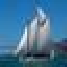
\includegraphics[]{figures/CIFAR10_example_3.pdf}}};

\end{tikzpicture}

